\section{User guides}

\subsection{Electronics}
To supply the system connect a suitable power source. The source should deliver 22-24V with atleast 0.5A to start the system. More amperage is needed to run the motors. Connect the supply to the connectors in the center of the bottom of the power board. The connectors are marked \texttt{IN EXT2}, \texttt{IN EXT1}, \texttt{IN BAT1} and \texttt{IN BAT2}. The source primarily used during the project has been a 6-cell Li-Po battery.

The BAT and EXT connectors share a common ground but are otherwise separated and the card will chose the voltage supply that have the highest potential. The EXT 1 and 2 and the BAT 1 and 2 are connected in parallel to each other respectively. To be able to start the whole system a MCU CAN-card with suitable software to control the system need to be mounted on the PSU-card. In order to start the motor supply and the 12 V supply the kill-switch need to be activated as well. 

The second significant part of the system is the CAN bus. The bus consists of several MCU CAN-cards connected to each other. Most of these connections are aided with the help of stack cards in the robot. These consists of a card with two six pin TP cable connectors, one power-supply connector and eight four pin bottom entry break away socket headers. The TP connectors connect the different stacks as well as supply the stacks later in the chain with power to supply the cards. \emph{One} of the stacks in the chain needs to be connected to one of the top three connectors on the right side of the power-board to the green connector on the bottom of the stack. The rest of the stacks are supplied via the TP cable. 

On the top half of the card there are the eight four pin bottom entry break away socket headers. The socket headers is where the MCU CAN-cards are to be connected. Make sure that the card goes \emph{through} the card \emph{first}. The breakaway header on the MCU CAN-card need to be angled and longer than standard to make a secure fit. They need to go all the way though to the other side and show at least a couple of millimetres on the back. 

The MCU CAN-cards have several extension boards to add functionality to the system. What these do and how they work are discussed in its respected sections. 

The brain of the robot is the beagle bone black (BBB). They are supplied by the power board and should be connected to the third and fourth connector on the left side from the top. This supply also need to be activated by the MCU CAN-card mounted on the power board. The BBB is also connected to the CAN bus via small card. This card changes the logical level from 5V in the CAN-cards to 3.3V that the BBB are using.  

The final cards are the GIMME 2 cards. These should be connected to the GIMMIE 2 power board. This is then connected to the same supply as the CAN bus, one of the top three connectors on the right side of the power-board.  

\subsection{Mechanics}
 \noindent This section will describe how to prepare the mechanical parts of Naiad for underwater use and how to handle the robot afterwards. It also goes through how to connect cables through the main hull and how to modify the length of an O-ring.
 	 \subsubsection{Preparation for Underwater Usage}
 	 \label{hullmanual}
	\noindent This section describes the steps to be done when preparing Naiad for use in water. Step 2-3 can be done either before or after the electronics have been placed into Naiad. However, to decrease the risk of accidental damage to the O-ring when adding the electronics, it is preferred to do it after all the electronics have been fitted.

\begin{enumerate}
  \item Make sure the insides of the main hull and lid are dry.
  \item Clean the O-ring track on the main hull with a wet towel or a piece of tissue and make sure the track is free from any dust or small hair. 
  \item Add a small amount of petroleum jelly along the whole track. 
  \item Clean the O-ring in the same manner as the O-ring track. It is important to check for any damage on the O-ring. Check for any cuts, dents or similar while cleaning it. Replace if it is damaged.
  \item Add a layer of petroleum jelly to the O-ring and make sure no hairs or dust gets stuck on it.
  
  \item Put the O-ring into the track. Make sure that the O-ring fits and is not too large. Preferably, the O-ring should be lying against the inner wall of the track. If it lies too much against the outer wall there is a high risk of it coming out of the track when, for example, putting on the lid. For more details about changing the size of the O-ring, see Section \ref{Oring}. 
\item	Attach the lid to the hull. Make sure all compressing spring latches are firmly closed. Make sure that the lid is put on straight from above rather than slided into place, since this might cause the O-ring to come out of its track.  
\item Make sure the kill and mission switches are mounted on the side of the hull. When in the water, the kill switch is to be removed when there is an emergency and Naiad needs to stop. The mission switch is to be removed for starting missions. 
\item Mount the front tool plate to the underside of the main hull in the very front to the pre-made holes with screws and nuts. Naiad is now ready to be put into water.
\end{enumerate}

	\subsubsection{Post-usage}
	\noindent After Naiad has been into water, the following steps should be done (where step 3-4 can be done before or after removing the electronics):
	
	\begin{enumerate}
	\item Dry the outside of Naiad to eliminate the risk of accidentally dripping water into the hull when removing the lid.
	\item Remove the lid and prevent damage to the O-ring by lifting the lid straight up.
	\item Remove the O-ring and clean it from the petroleum jelly with a piece of tissue. 
	\item Clean the O-ring track free from the petroleum jelly.
	\item On every thruster: Locate the screw on top of the thruster, just beneath the propeller. Unscrew it. See fig. \ref{happs} for the location of the screws.
	
	\begin{figure}[!ht]
	\begin{center}
		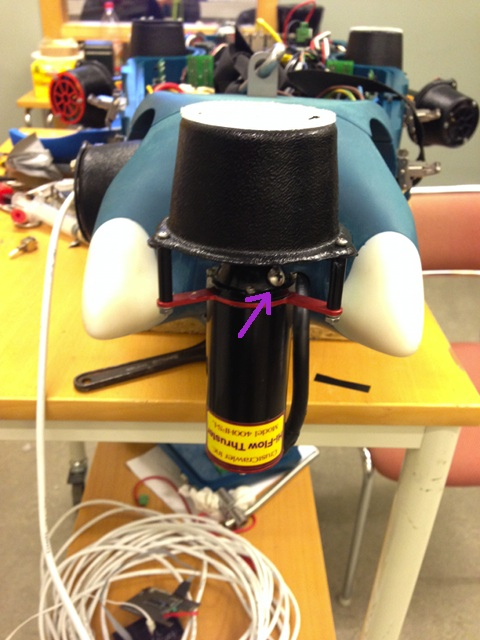
\includegraphics[width=85mm]{./Images/Mechanics/ThrusterScrew.jpg}
		\caption{The location of the screw for grease refilling.}
		\label{happs}
	\end{center}
\end{figure}
	
	For the horizontal thruster in the very back of Naiad, first remove the two, horizontally placed, small screws on the part that covers the motor. Then unscrew the two screws that go vertically straight through from the top. Carefully remove the covering part. Unscrew the screw on the thruster. The placement of the screws can be seen in fig. \ref{hellus}.
	 
	 \begin{figure}[!ht]
	\begin{center}
		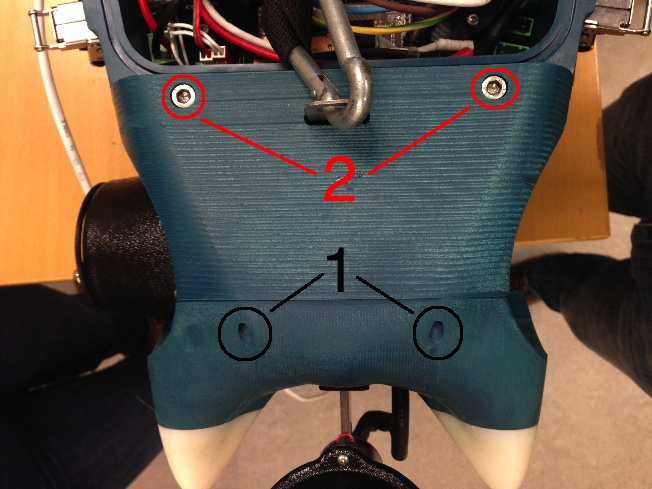
\includegraphics[width=85mm]{./Images/Mechanics/ScrewsThrusterCover.jpg}
		\caption{The two sets of screws for accessing the rear motor. Number 1 indicates the horizontal screws and Number 2 indicates the vertical screws.}
		\label{hellus}
	\end{center}
\end{figure}
	 
	\item Add grease in a large syringe.
	\item Insert the syringe into the screw holes and inject grease until some grease comes out of the top of the thruster and any water has been pushed out. Repeat for all six motors. 
	\item Put all the screws back on the thrusters. For the covered thruster in the back, put the cover back on in reversed order from step 5.
	\end{enumerate}
	
	\subsubsection{Adaptions to the system}
	The following section describes optional configurations of Naiad. 
	\subsubsection*{Connecting Cables}
	\label{Connecting}
	\noindent Naiad can be equipped with equipment that may need to be connected to the electronics inside of the hull. This section describes how to manage this.
	\begin{enumerate}
	\item Locate the four plugs in the bottom of the main hull. Remove the plug of any of the four holes that is closest to the peripheral that needs to be connected to inside of the hull.
	\item Insert the cable through a cable gland and then through the hole in the hull.
	\item tighten the cable gland on the outside and put on a screw nut from the inside. Make sure not to tighten the cable gland too much as it could damage the hull.  
	\end{enumerate}
	
	\subsubsection*{Adjusting the length of the O-ring}
	\label{Oring} 
	\noindent If the O-ring is too large for the main hull, do the following steps in order to make it fit (if making a new O-ring, start from step 2):
	
	\begin{enumerate}
	\item Cut off the O-ring as perpendicular and straight as possible, to get nice and clean endings.
	\item Put glue, preferably special O-ring glue, on both ends of the O-ring and then put the ends together.
	\item Wait for the glue to dry and then check if the splicing is secured. 
	\end{enumerate}
	It is highly recommended to put Naiad with the new O-ring in water without electronics to check the quality of the O-ring repair.  
	